\chapter{Theorie}
\label{cha:theorie}
Als Grundlage für die nachfolgenden Kapitel, wird in diesem Kapitel die Theorie hinter den verschiedenen Arbeitsschritten zur Sprechererkennung vorgestellt. Dies erfolgt in der Reihenfolge, wie die einzelnen Schritte verwendet werden. Die Reihenfolge geht aus dem Abschnitt \ref{sec:uebersicht} hervor.

\section{Übersicht}
\label{sec:uebersicht}
Die Sprechererkennung und auch weitere Anwendungen wie Sprecherverfikation, Gesichtserkennung und Texterkennung, werden jeweils in vier Arbeitsschritte unterteilt. Diese sind \emph{Preprocessing}, \emph{Training}, \emph{Prediction} und \emph{Analysis}. Diese werden, so wie in Abbildung \ref{fig:allgemeinerAblauf} dargestellt, nacheinander ausgeführt. Beim Preprocessing (engl.: Vorverarbeitung) werden die Daten in das passende Format konvertiert, wichtige Informationen extrahiert und eventuell skaliert. Danach findet das Training durch einen Klassifikator oder ein künstliches neuronales Netz statt. Die Prediction (engl.: Vorhersage) ist die eigentliche Arbeitsphase der Erkennung. Anhand der trainierten Daten wird entschieden, welchem Sprecher die eingegeben Daten zugeordnet werden können. Der letzte Arbeitsschritt stellt die Analysis (engl. Analyse) dar. Hierdurch werden die Ergebnisse der Prediction verifiziert und evtl. auch visualisiert.

\begin{figure}[h]
  \centering
  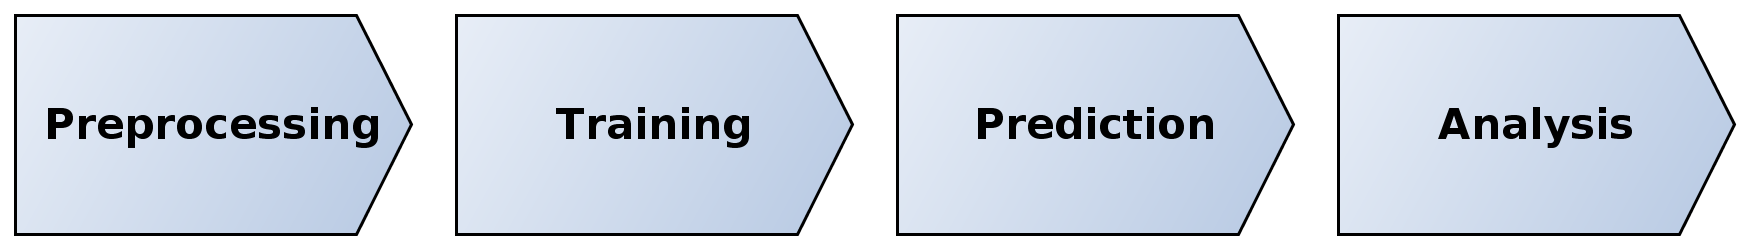
\includegraphics[width=0.85\textwidth]{images/allgemeinerAblauf}
  \caption{Einzelne Arbeitsschritte der Sprechererkennung}
  \label{fig:allgemeinerAblauf}
\end{figure}

\section{Preprocessing}
Der Schritt der Vorverarbeitung teilt sich in drei Teile auf: \emph{Konvertierung}, \emph{Feature Extraction} und \emph{Skalierung}. Diese drei Schritte werden in den folgenden Abschnitten genauer erläutert. Das Preprocessing ist von der Problemstellung abhängig. Bei der Sprechererkennung ist es die Verarbeitung von Audiostreams und die Abbildung auf die Stimm- und Hörorgane des Menschen.

\subsection{Konvertierung}
Mit der Konvertierung wird dafür gesorgt, dass die Daten im gleichen Format vorliegen. Für die Sprechererkennung reicht es, wenn die Audiodaten auf einen Kanal beschränkt werden (\emph{Mono}). Des Weiteren wird in dieser Projektarbeit eine Abtastrate von 16 kHz und einer Abtastgenauigkeit von 16 Bit verwendet.

\subsection{Feature Extraction}
Zur Extraktion von wichtigen Informationen werden zwei gängige Verfahren eingesetzt. Zum einen ist dies das Linear Predictive Coding (LPC). Beim LPC wird der Stimmtrakt des Menschen modellhaft nachgebildet. Dadurch wird die Datenbasis stark reduziert und nur die wichtigsten Informationen werden gespeichert. Zum anderen werden Mel Frequency Cepstral Coefficients (MFCC) eingesetzt. Diese sollen an das menschliche Gehör angelehnt sein und bilden dadurch die menschliche Wahrnehmung nach.

\subsection{Skalierung}
Gelegentlich kann durch eine Skalierung der extrahierten Daten die Erkennung verbessert werden. Wahlweise kann zwischen $[0,1]$ oder $[-1,1]$ skaliert werden. Die Skalierung erfolgt linear nach der Formel \ref{equ:skalierung1} für $[0,1]$ und nach der Formel \ref{equ:skalierung2} für $[-1,1]$. $min$ stellt den kleinsten Wert der zu skalierenden Daten dar. $max$ den größten Wert. \cite{bib:svmfaq}
\begin{equation}
	\label{equ:skalierung1}
	x'=\frac{x-min}{max-min}
\end{equation}
\begin{equation}
	\label{equ:skalierung2}
	x'=2*\frac{x-min}{max-min}-1
\end{equation}

\section{Training}
Für die Trainingsphase werden in dem Projekt \emph{Neural Gas}, ein Verfahren zur Clusteranalyse, und der Klassifikator \emph{Support Vector Machine} eingesetzt. 

\subsection{Neural Gas}
Neural Gas, eine Variante von selbstorganisierende Karten, gilt als ein sehr robustes neuronales Netz. Da im Gegensatz zu K-Means auch eine Nachbarschaftsreichweite in Neural Gas eingeführt wird, wird eine Konvergenz auch nahezu unabhängig von der Initalisierung erreicht. \cite{bib:neuralGas} Die Update-Regel, die für einzelne Clusterprototypen gilt, lautet wie in Formel \ref{equ:neuralGas} beschrieben.

\begin{equation}
	\label{equ:neuralGas}
	\begin{aligned}[t]\Delta w_{i} = \epsilon(t) * e^{-k_i / \lambda(t)} * \left(x - w_i\right)\end{aligned}
\end{equation}

$\epsilon(t)$ stellt hierbei die Lernrate dar. Diese sollte über die Zeit absteigend sein um Sprünge nur am Anfang des Trainings zu erlauben. In diesem Projekt wurde die Lernrate nach Formel \ref{equ:neuralGasLernrate} gewählt, wobei $\epsilon_\text{start} = 1$ und $\epsilon_\text{end} = 0,001$ gesetzt wurden.

\begin{equation}
	\label{equ:neuralGasLernrate}
	\epsilon(t) = \epsilon_\text{start} \cdot \left( \frac{\epsilon_\text{end}} {\epsilon_\text{start}} \right) ^ {\frac{t}{t_{\text{max}}}}
\end{equation}

Bei der Nachbarschaftsreichweite wurde die Formel \ref{equ:neuralGasNachbar} mit $\lambda_\text{start} = N/2$ und $\lambda_\text{end} = 0,01$ eingesetzt. $N$ ist die Anzahl der Merkmalsvektoren, die für das Verfahren eingesetzt werden.

\begin{equation}
	\label{equ:neuralGasNachbar}
	 \lambda(t) = \lambda_\text{start} \cdot \left( \frac{\lambda_\text{end}} {\lambda_\text{start}} \right) ^ {\frac{t}{t_{\text{max}}}}
\end{equation}


\subsection{Support Vector Machine}
Eine Support Vector Machine (SVM) ist ein Klassifikator der zur Mustererkennung eingesetzt wird. Eine SVM ermittelt eine Trennebene zwischen zwei Mengen, die diese Mengen optimal, also mit möglichst großem Abstand (\emph{Trennspanne}) zu allen Punkten, teilt. Falsch klassifizierte Datenpunkte werden als Strafpunkte angerechnet. Hierbei wird der Abstand mit dem Fehlergewicht $C$ multipliziert. Bildlich dargestellt wird das Verfahren in Abbildung \ref{fig:svmA}. Hierbei ist stellt die durchgezogene Linie die Trennebene dar, die gestrichelte Linie die Trennspanne und die gekreuzten Punkte sind falsch klassifizierte Punkte.

\begin{figure}[h]
  \centering
  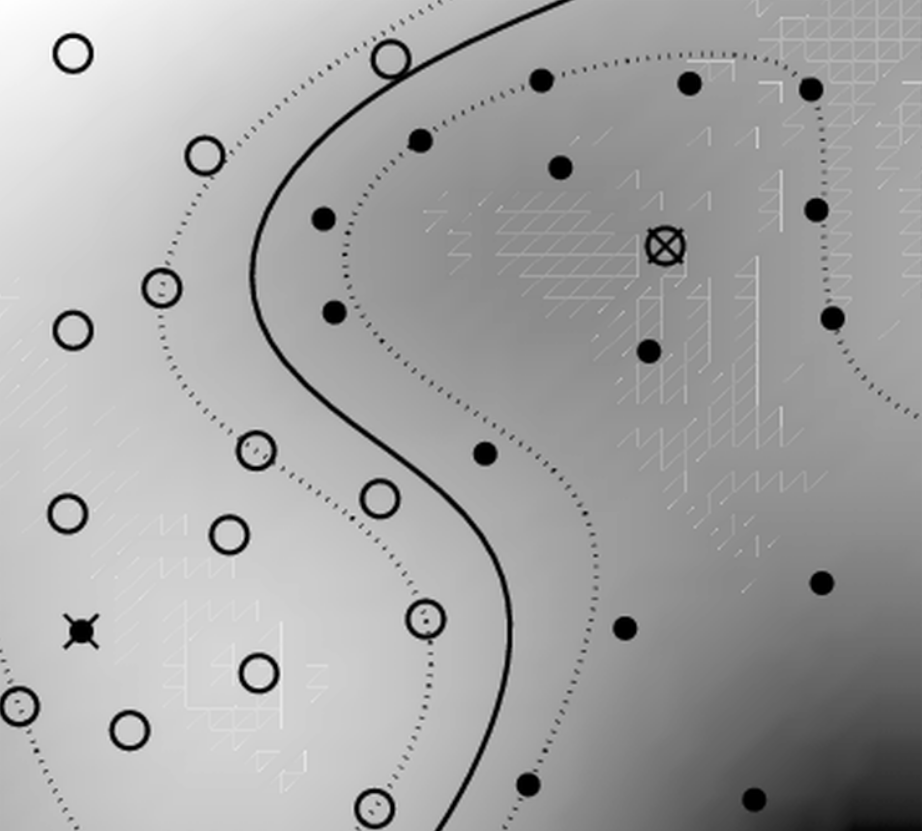
\includegraphics[width=0.65\textwidth]{images/svmA}
  \caption{Beispiel einer Klassifikation mit SVM \cite[S. 217]{bib:svmA}}
  \label{fig:svmA}
\end{figure}

Um falsch klassifizierten Punkte in Abbildung \ref{fig:svmA} ebenfalls korrekt zu klassifizieren muss das Klassifikationsproblem höherdimensional betrachtet werden. Somit kann eine Hyperebene gefunden werden, die das Problem korrekt klassifiziert. Statt dem Skalarprodukt als Distanzfunktion werden Kernels verwendet. Im Projekt werden hier lineare Kernel und radiale basisfunktionale Kernel (RBF) verwendet. Zum oben genannten Beispiel kann ein korrekt klassifiziertes Problem wie in Abbildung \ref{fig:svmB} aussehen.

\begin{figure}[h]
  \centering
  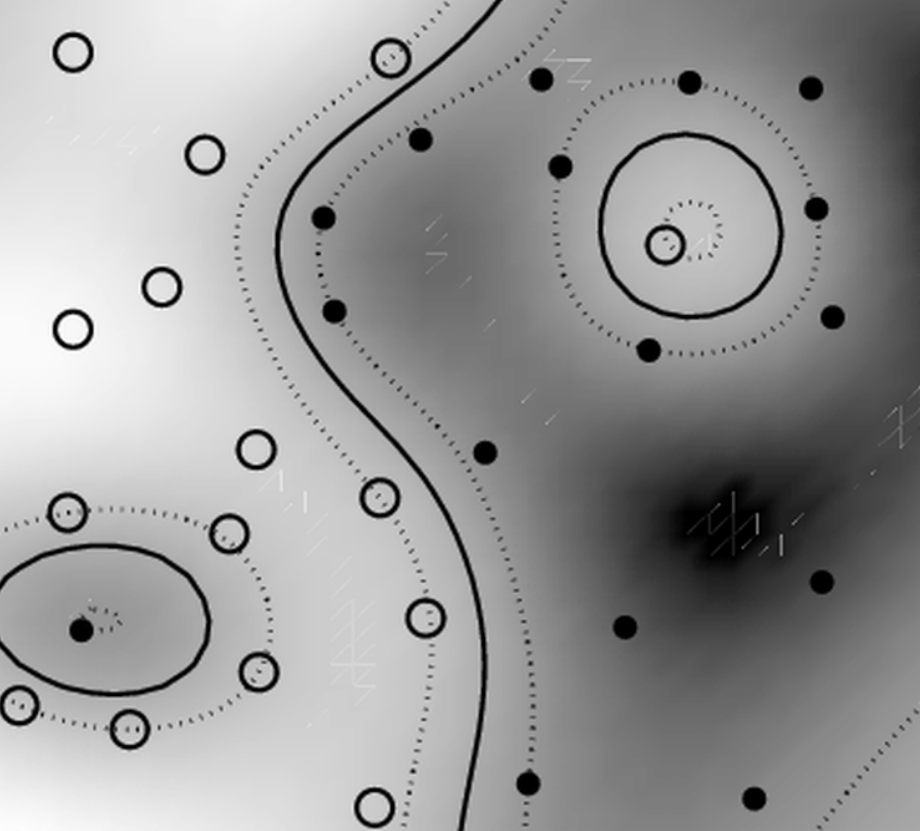
\includegraphics[width=0.65\textwidth]{images/svmB}
  \caption{Klassifikation mit SVM im höherdimensionalen Raum \cite[S. 217]{bib:svmA}}
  \label{fig:svmB}
\end{figure}

Um die Klassifikation mit SVM auf mehrere Mengen anzuwenden, können zwei Verfahren angewendet werden. Zum einen \emph{one-against-one}, d.h. es werden Trennebenen zwischen allen möglichen Mengenpaaren ermittelt. Zum anderen \emph{one-against-all}, d.h. es wird immer eine Menge zu allen anderen Punkten abgegrenzt. In diesem Projekt wird die \emph{libsvm} und damit \emph{one-against-one} eingesetzt, da diese Methode schneller trainiert. \cite{bib:svmB}

\section{Prediction}
Bei der Prediction handelt es sich um die eigentliche Arbeitsphase der Sprechererkennung. Dabei wird in den trainierten Daten gesucht, ob ein vorliegendes Eingangssignal mit einer trainierten Klasse übereinstimmt. Die Ergebnisse werden dann an die Analyse weitergereicht um zu ermitteln, wie wahrscheinlich es ist, den richtigen Sprecher erkannt zu haben.

Es werden zwei Methoden für die Predicition in diesem Projekt verwendet. Die erste ist die \emph{Nearest Neighbor}-Methode (engl.: nächster Nachbar) und schaut in einem Codebuch nach dem passensten Eintrag. Somit eignet er sich um die Ergebnisse des Neural Gas Algorithmus zu verarbeiten. Die zweite Methode ist die Klassifikation mittels SVM.

\subsection{Nearest Neighbor}
Bei der \emph{Nearest Neighbor}-Methode wird nach dem Codebuchvektor gesucht, der die geringste Distanz zum Eingabevektor aufweist. Hierbei wird wie in Formel \ref{equ:nearestNeighbor} die euklidische Distanzen ermittelt. In der Praxis wird allerdings auf die Wurzel verzichtet, da die Reihenfolge der Distanzen gleich bleibt und somit auf diesen Rechenaufwand verzichtet werden kann.

\begin{equation}
	\label{equ:nearestNeighbor}
	d(x,y) = \|x-y\|_2 = \sqrt{\sum_{i=1}^n (x_i-y_i)^2}
\end{equation}

\subsection{Klassifikation mittels SVM}
Um den Eingabevektor in dem mit SVM erstellte Modell einzuordnen wird eine einfache Klassifikation durchgeführt. Hierbei wird wieder das \emph{one-against-one}-Verfahren eingesetzt um zu entscheiden welcher der Trainingsvektormengen der Eingabevektor zugeordnet werden kann.

\section{Analysis}
Die Predicition liefert Einzelergebnisse, die alleine nur wenig Aussagekraft über die eingesetzten Methoden besitzen. Möchte man die Wahrscheinlichkeit errechnen, mit der der angegebene Sprecher wirklich spricht, müssen Analysen mit den Testdaten ausgeführt werden. Als Test bietet sich die \emph{Cross-Validation}-Methode an. Hierbei werden die Testdaten in nahezu gleichgroße Blöcke unterteilt. Ein Block wird zum Testen und der Rest zum Trainieren verwendet. Das wird so oft wiederholt bis jeder Block einmal als Testblock verwendet wurde. Um nun die Wahrscheinlichkeit der richtigen Klassifizierung anzugeben bietet sich beispielweise die absolute Erkennungsrate an. Diese ist die Anzahl der korrekt erkannten Frames dividiert durch die Anzahl der Gesamtframes. Eine weitere Methode zur Analyse stellt die Verwechslungsmatrix dar. Diese kann einfach visualisiert werden und zeigt an, welche Sprecher oft falsch klassifiziert oder gar verwechselt werden. Auf einer Achse der Matrix wird der erkannte Sprecher angegeben, auf der anderen Achse der tatsächliche Sprecher.


